\section{Methodology}
\label{sec:methodology}

Since we have three members, we decided to tackle the project by assigning a machine learning model to each member. Chathumini focused on creating the Logistic Regression model, while also exploring the differences between batch and stochastic gradient descent and implementing k-fold cross validation. Saadiya worked on creating the SVM model and plotting their Precision-Recall Curves. Kevin implemented the ID3 and Random Forest models, compared their yielded metrics, and determined the most important features.

\subsection{Exploratory Data Analysis and Feature Engineering}
\label{sec:methodology:Exploratory Data Analysis and Feature Engineering}

Before we started creating any models, we collectively worked on the Exploratory Data Analysis (EDA) of the stroke risk dataset. For EDA, we plotted histograms and a heatmap to visualize the data and the correlation between the features. Through EDA, we learned that there were some missing values for certain features, unnecessary columns, categorical variables, and most importantly, that there was an imbalance in the data in terms of the stroke feature. Figures \ref{fig:Figure1} and \ref{fig:Figure2} show how the data distribution was initially:

\begin{figure}[ht]
    \centering
    \begin{subfigure}[t]{0.4\textwidth}
        \centering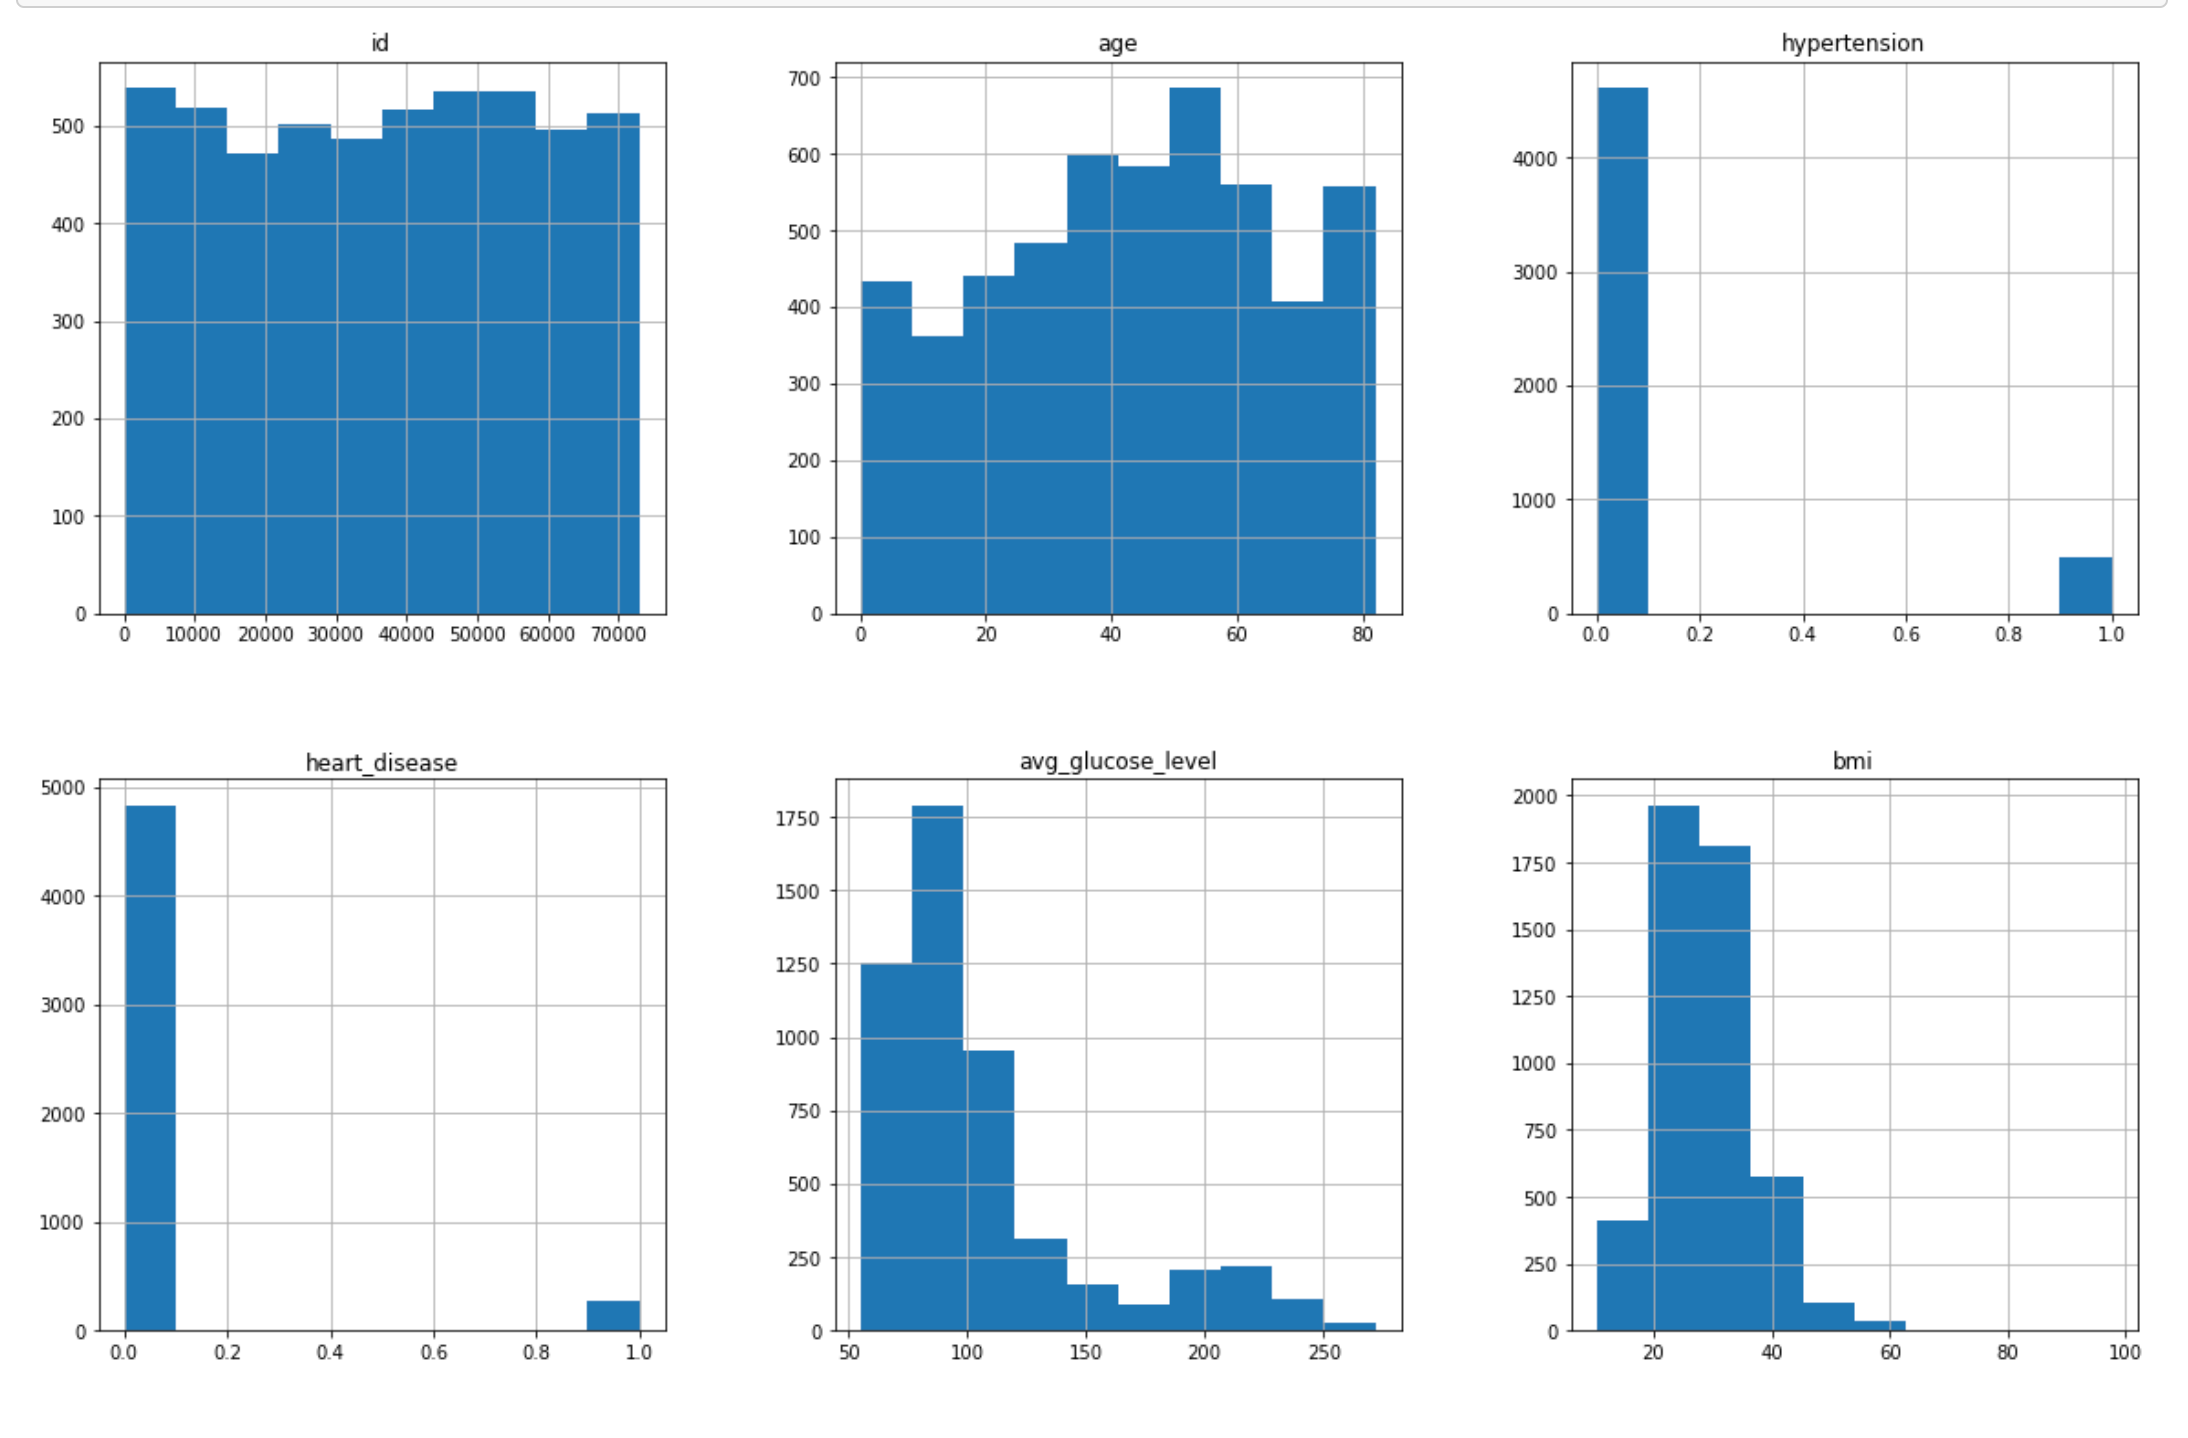
\includegraphics[width=1\linewidth]{Data1}
        \caption{Initial Feature Distribution}
        \label{fig:Figure1}
    \end{subfigure}
    \begin{subfigure}[t]{0.3\textwidth}
        \centering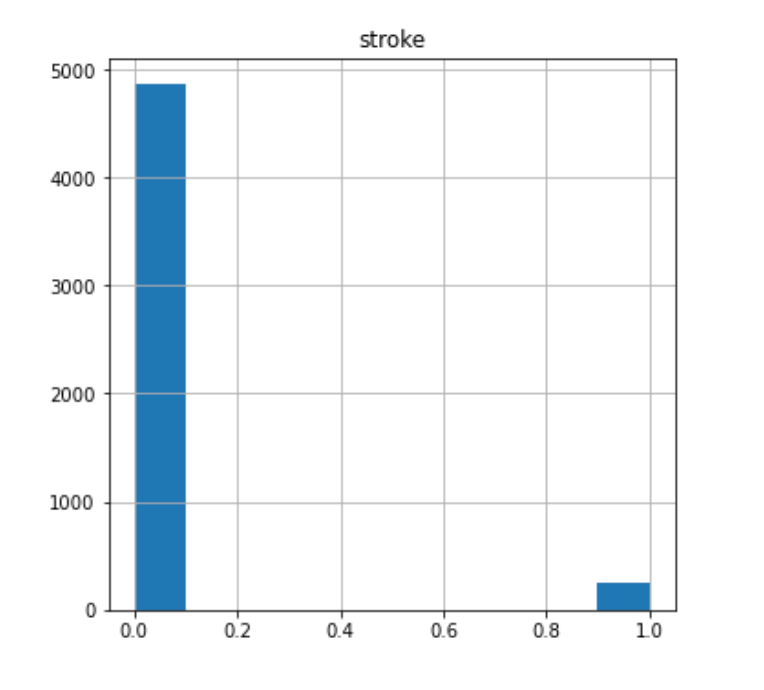
\includegraphics[width=1\linewidth]{Data2}
        \caption{Initial Label Distribution}
        \label{fig:Figure2}
    \end{subfigure}
\end{figure}

\noindent To fix these issues, we performed feature engineering \cite{Stroke_Prediction}. We filled the missing values with that features average result and discarded any unnecessary columns. We then changed the categorical data to numerical data. To fix the imbalance issue, we used the Synthetic Minority Oversampling Technique (SMOTE), which works by selecting examples that are close in the feature spaces, draws a line between the examples in the feature space, and draws a new sample at a point along that line. We also standardized the data by computing the following equation on our features $X$:

\begin{equation}
    \label{eq:Equation1}
    X_{standardized} = \dfrac{X - \mu(X)}{\sigma(X)}
\end{equation}

Where $\mu(X)$ is the mean of $X$, and $\sigma(X)$ is the standard deviation of $X$.\\

\noindent Figures \ref{fig:Figure3} and \ref{fig:Figure4} show feature correlations before and after: replacing N/A values, converting categorical data to discrete data, and standardizing data using Equation \eqref{eq:Equation1}:

\begin{figure}[H]
    \centering
    \begin{subfigure}[t]{.85\textwidth}
        \centering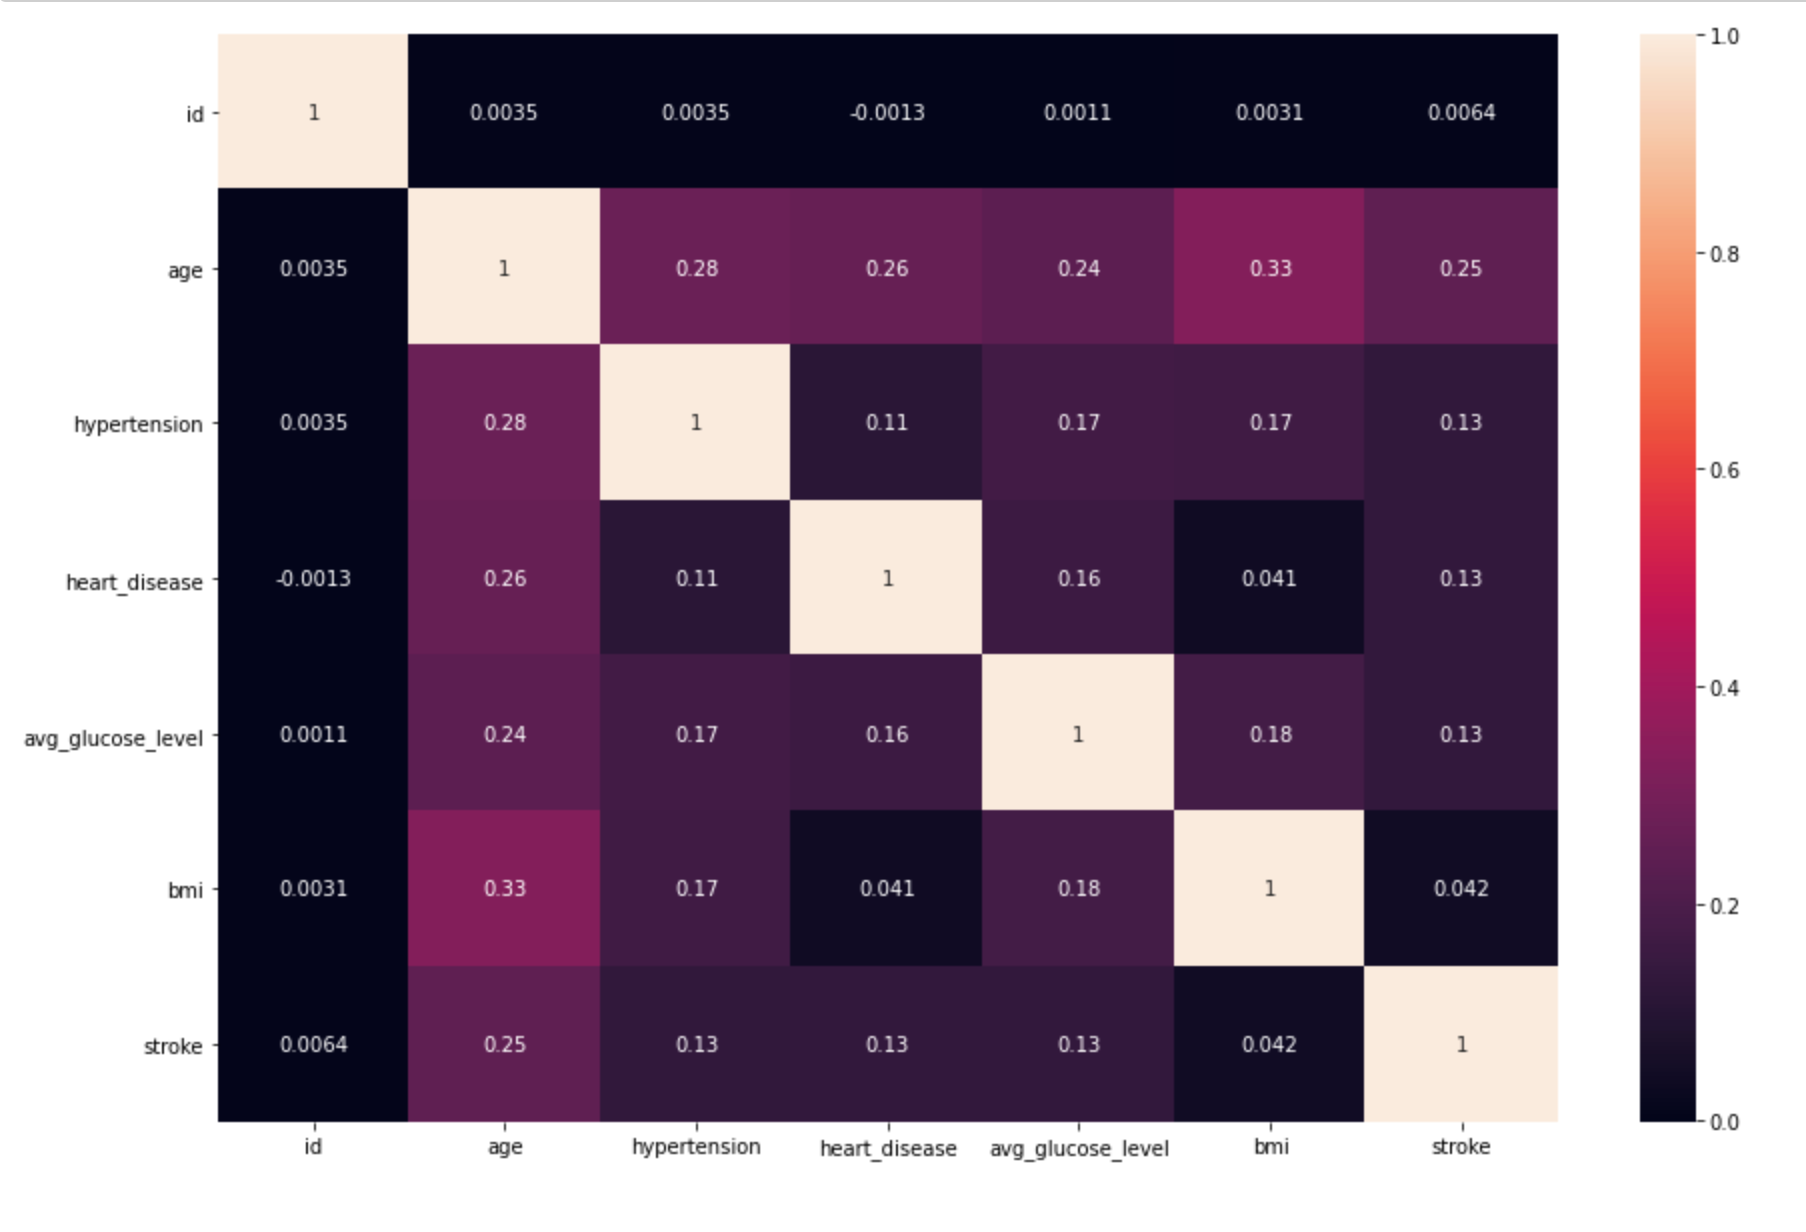
\includegraphics[width=1\linewidth]{Data3}
        \caption{Initial Covariance Matrix}
        \label{fig:Figure3}
    \end{subfigure}\\
    \begin{subfigure}[t]{.85\textwidth}
        \centering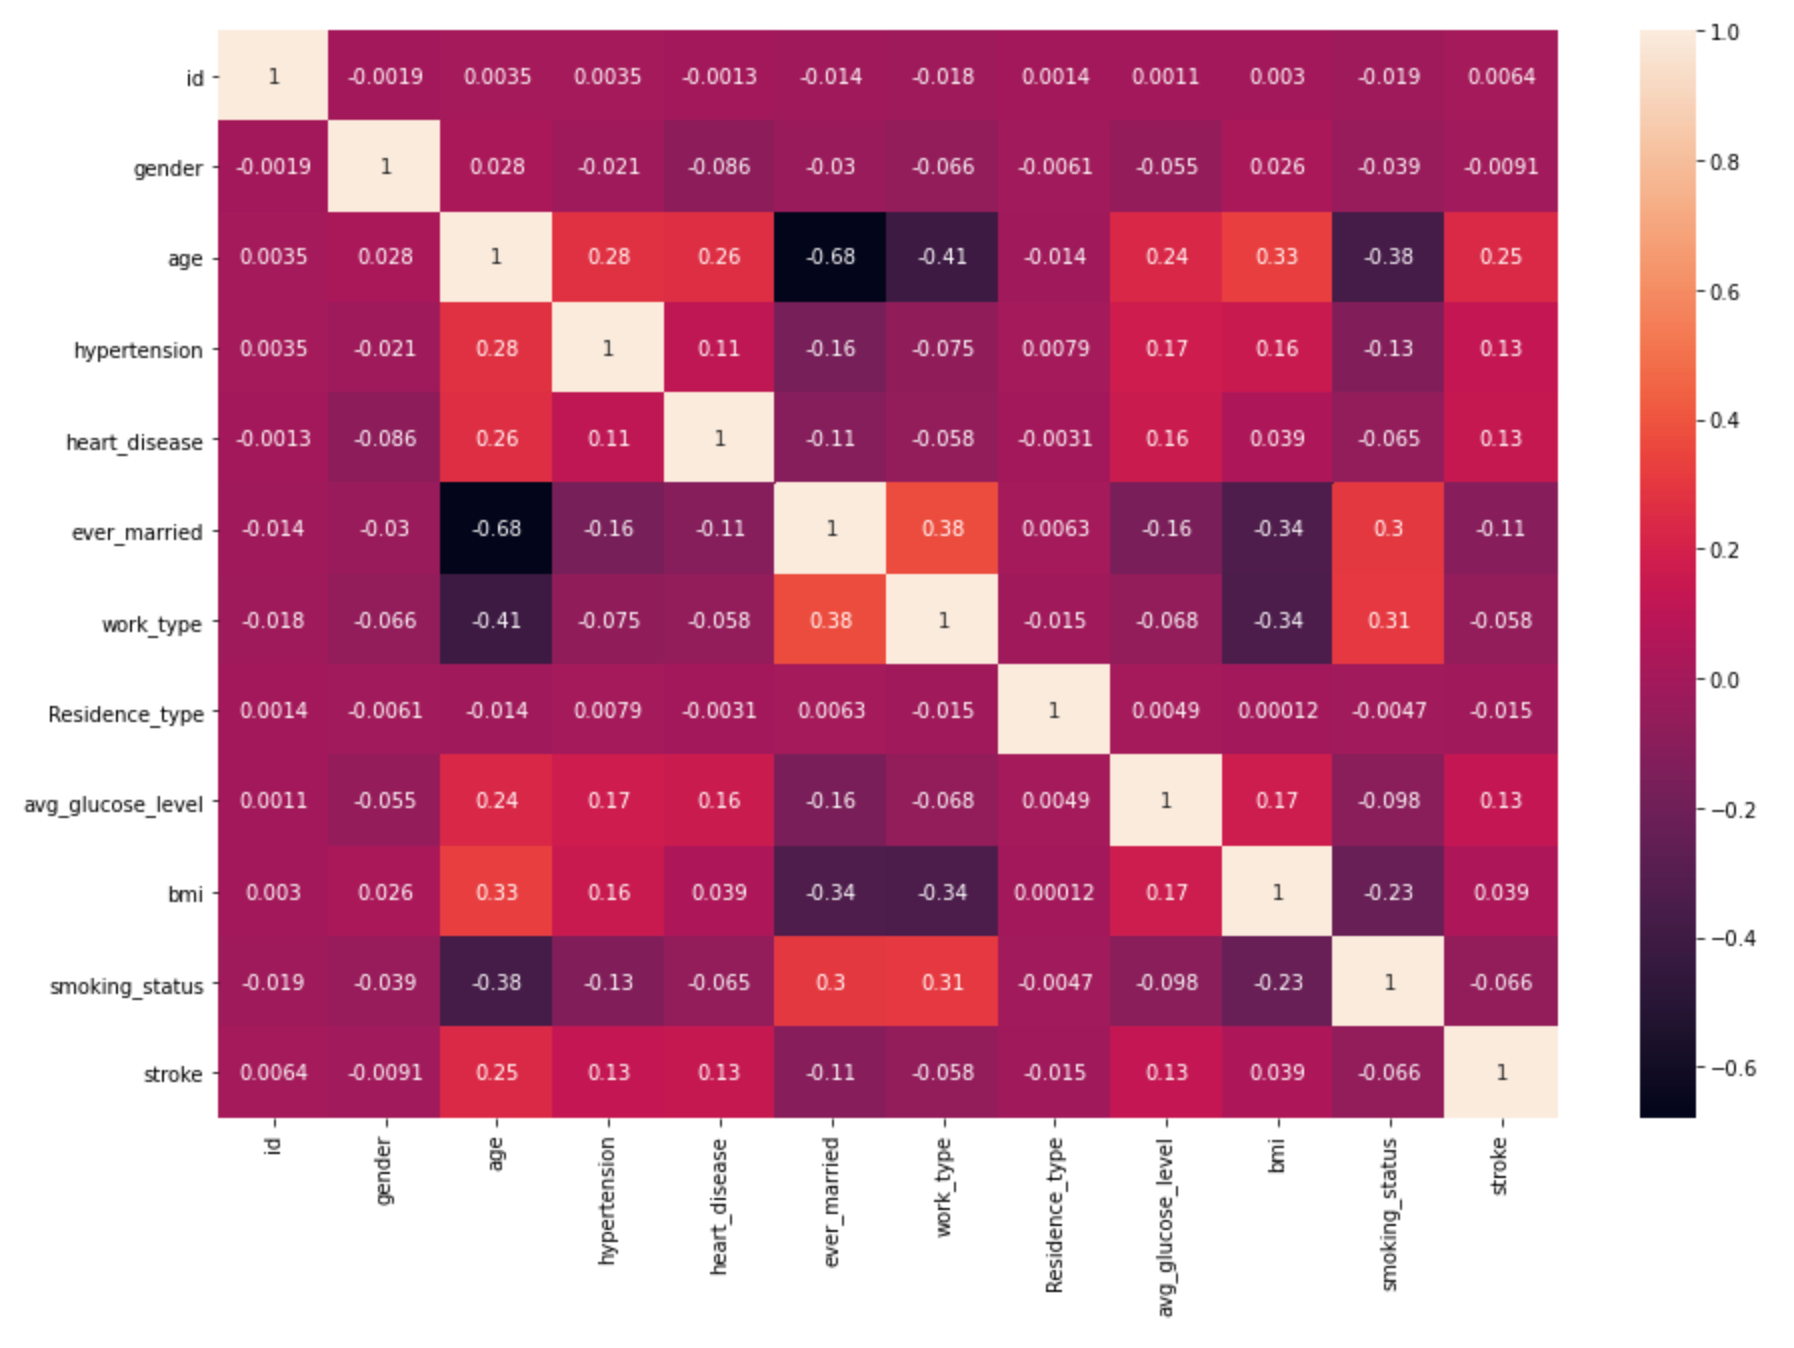
\includegraphics[width=1\linewidth]{Data4}
        \caption{Final Covariance Matrix}
        \label{fig:Figure4}
    \end{subfigure}
\end{figure}

\subsection{Picking Models}
\label{sec:methodology:Picking Models}

With the feature engineering and SMOTE applied to the data, we are ready to proceed. Given the nature of the data, we are facing a supervised learning problem, more specifically a classification problem. Given the severity of the issue at hand, we wanted to compare some more basic classification algorithms, like Logistic Regression \cite{Logistic_Regression}, and see how it would fare against different discriminative algorithms such as SVMs \cite{SVMs} and Decision Trees. In addition, we wanted to find out which features mattered the most in this case, which is the Random Forest algorithm was picked out of all possible Decision Tree based algorithms. 